\documentclass[12pt]{article}
\setlength{\oddsidemargin}{0in}
\setlength{\evensidemargin}{0in}
\setlength{\textwidth}{6.5in}
\setlength{\parindent}{0in}
\setlength{\parskip}{\baselineskip}

\usepackage{amsmath,amsfonts,amssymb,graphicx,xcolor,mathtools}

\newcommand{\purple}[1]{{\color{purple} #1}}

\begin{document}

PHYS 374 Fall 2020\hfill Worksheet 6: Hanging Chain\\
\\
Name: \purple{SOLUTION}\\
\\
Please submit as a PDF on Moodle. Include any calculations made using external tools.

\hrulefill
\\
\\
Two rigid posts of height $H$ stand at $x=-L$ and $x=L$. A chain of length $\ell$ hangs between them. The mass of the chain, $m$, is uniformly distributed along its length.
\begin{enumerate}
\item Draw a picture!
\item Write down the potential energy of a small section of the chain $dm$, then write down an integral over $dm$ for the potential energy of the entire chain.
\item Rearrange your potential energy integral into rectangular coordinates. 
\item The length of the chain is fixed. Write down that constraint as another integral, then rearrange it into the same coordinates as above.
\item Combine your two integrals into a single expression using a Lagrange multiplier $\lambda$.
\item Use the Euler-Lagrange equation to find a differential equation describing the chain.

Hint: recall when $f(y, y', x)$ doesn't depend on $x$, the EL equation can be rewritten: 
$$
\frac{\partial f}{\partial y} - \frac{d}{dx} \frac{\partial f}{\partial y'} = 0
\quad\quad\rightarrow\quad\quad
f - y' \frac{\partial f}{\partial y'} = \text{constant}
$$
\item Solve the differential equation to get an expression $y(x)$.

Hint: try the substitution $\cosh u = \alpha y + \beta$, where $\alpha$ and $\beta$ are constants. Note also:
\begin{align*}
    \tfrac{d}{du} \cosh u &= \sinh u&
    \tfrac{d}{du} \sinh u &= \cosh u&
    \cosh^2 u - \sinh^2 u &= 1
\end{align*}
\item Explain the significance of any undetermined constants in your expression $y(x)$. Give a simple expression relating each constant to known quantities (you do not need to solve those expressions). 
\end{enumerate}

\newpage

\purple{

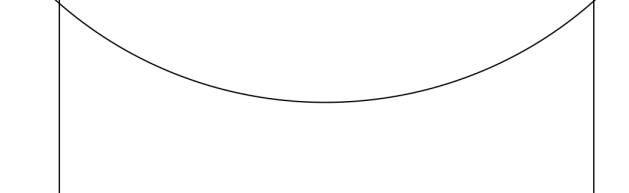
\includegraphics[width=5cm]{hanging-chain.png}

TODO: add diagram here

The potential energy of a small section of chain is:
$$
dU = dm \; g y
$$
Which we can integrate over the length of the chain to get:
$$
U = \displaystyle \int_{-L}^L dU = \displaystyle \int_{-L}^L dm \; g y
$$
The mass is distributed uniformly over the length of the chain (rather than being distributed uniformly in the horizontal direction) so:
$$
dm = \mu \; d\ell = \mu \sqrt{dx^2 + dy^2} = \mu \; dx \; \sqrt{1 + y'^2} 
$$
Where $\mu$ is the chain mass density $\mu = \tfrac{m}{\ell}$ and $y' = \tfrac{dy}{dx}$.

Then:
$$
U = \displaystyle \int_{-L}^L dx \; \mu g y \sqrt{1 + y'^2} 
$$
Similarly, we can write the constraint as:
$$
\ell = \displaystyle \int d\ell = \displaystyle \int_{-L}^L \sqrt{dx^2 + dy^2} = \displaystyle \int_{-L}^L dx \; \sqrt{1 + y'^2}
$$
Combining these two expressions with the help of a Lagrange multiplier gives:
$$
U^* = U + \lambda \ell 
=
\displaystyle \int_{-L}^L dx \; \left[ \mu g y \sqrt{1 + y'^2} + \lambda \sqrt{1 + y'^2} \right]
$$
The integrand above is:
$$
f = (\mu g y + \lambda) \sqrt{1 + y'^2}
$$
This does not directly depend on $x$, so we can use a shorter version of the Euler-Lagrange equation (per the hint above). Note we use $k$ to represent the undetermined constant of integration:
$$
f - y' \frac{\partial f}{\partial y'} = k
\quad\rightarrow\quad
(\mu g y + \lambda) \sqrt{1 + y'^2} - y' (\mu g y + \lambda) \frac{y'}{\sqrt{1 + y'^2}} = k
$$
A bit of rearranging...
\begin{align*}
    (\mu g y + \lambda) \sqrt{1 + y'^2} - y' (\mu g y + \lambda) \frac{y'}{\sqrt{1 + y'^2}} &= k \\
    (\mu g y + \lambda) (1 + y'^2) - y'^2 (\mu g y + \lambda) &= k \sqrt{1 + y'^2} \\
    \mu g y + \lambda &= k \sqrt{1 + y'^2} \\
    (\mu g y + \lambda)^2 &= k^2 (1 + y'^2) \\
    \left( \frac{\mu g y + \lambda}{k} \right)^2 - 1 &= y'^2\\
    \sqrt{ \left( \frac{\mu g y + \lambda}{k} \right)^2 - 1 } &= y'\\
\end{align*}
Note that we have two undetermined constants, $\lambda$ and $k$. To save ourselves a bit of writing, we can rewrite using two new undetermined constants $\alpha = \tfrac{\mu g}{k}$ and $\beta = \tfrac{\lambda}{k}$. Then separation of variables:
\begin{align*}
    \sqrt{ \left( \alpha y + \beta \right)^2 - 1 } &= \frac{dy}{dx} \\
    dx &= \frac{dy}{ \sqrt{ \left( \alpha y + \beta \right)^2 - 1 } } \\
    \int dx &= \int \frac{dy}{ \sqrt{ \left( \alpha y + \beta \right)^2 - 1 } }
\end{align*}
Then a $u$ substitution:
\begin{align*}
    \cosh u &= \alpha y + \beta \\
    \sinh u \; du &= \alpha \; dy \\
    \tfrac{1}{\alpha} \sinh u &= dy \\
\end{align*}
Plugging that in we get:
\begin{align*}
    \int dx &= \int \frac{\tfrac{1}{\alpha} \sinh u \; du}{ \sqrt{ \cosh^2 u - 1 } } \\
    \int dx &= \tfrac{1}{\alpha} \int \frac{ \sinh u \; du}{ \sqrt{ \sinh^2 u } } \\
    \int dx &= \tfrac{1}{\alpha} \int \frac{ \sinh u \; du}{ \sinh u } \\
    \int dx &= \tfrac{1}{\alpha} \int du \\
    x &= \tfrac{1}{\alpha} ( u + \gamma ) = \tfrac{1}{\alpha} \cosh^{-1} ( \alpha y + \beta ) + \tfrac{\gamma}{\alpha}
\end{align*}
Where $\gamma$ is another constant of integration. Solving for $y$ as a function of $x$ we get:
$$
y(x)= \tfrac{1}{\alpha} \cosh ( \alpha x + \gamma ) - \tfrac{\beta}{\alpha}
$$
A curve of the form $y = \tfrac{1}{\alpha} \cosh \alpha x$ is called a catenary. This sort of curve pops us all the time in architecture. The parameter $\alpha$ describes the ``steepness" of the curve, while $\gamma$ is a horizontal offset and $\tfrac{\beta}{\alpha}$ is a vertical offset. 

We can then come up with expressions for $\alpha$, $\beta$, and $\gamma$ from the known quantities.

The lowest point of our curve is at $x=-\tfrac{\gamma}{\alpha}$, and it rises symmetrically from there (since $\cosh$ is an even function). So in order to have $y(-L) = y(L)$ the lowest point must be halfway between them at $x=0$.  That means:
$$
\gamma=0
$$
We can then determine $\alpha$ from our constraint. Note $y' = \sinh \alpha x$ so:
\begin{align*}
    \ell &= \displaystyle \int_{-L}^L dx \; \sqrt{1 + y'^2} \\
    \ell &= \displaystyle \int_{-L}^L dx \; \sqrt{1 + \sinh^2 \alpha x} \\
    \ell &= \displaystyle \int_{-L}^L dx \; \cosh \alpha x \\
    \ell &= \Big[ \tfrac{1}{\alpha} \sinh \alpha x \Big|_{-L}^L \\
    \ell &= \tfrac{1}{\alpha} \sinh ( \alpha L ) - \tfrac{1}{\alpha} \sinh ( -\alpha L )\\      
    \ell &= \tfrac{2}{\alpha} \sinh (\alpha L) \\
\end{align*}
This expression cannot be solved analytically, but once we have $L$ and $\ell$ we can numerically solve for $\alpha$.

Finally, we can figure out $\beta$ from $y(L) = H$:
$$
H = \tfrac{1}{\alpha} \cosh ( \alpha L ) - \tfrac{\beta}{\alpha}
$$
Once we have $H$ and $\alpha$, we can use this relationship to get $\beta$.
}


\end{document}